\documentclass [tikz] {standalone}

%common figure styles
\input{header.htex}

\begin {document}



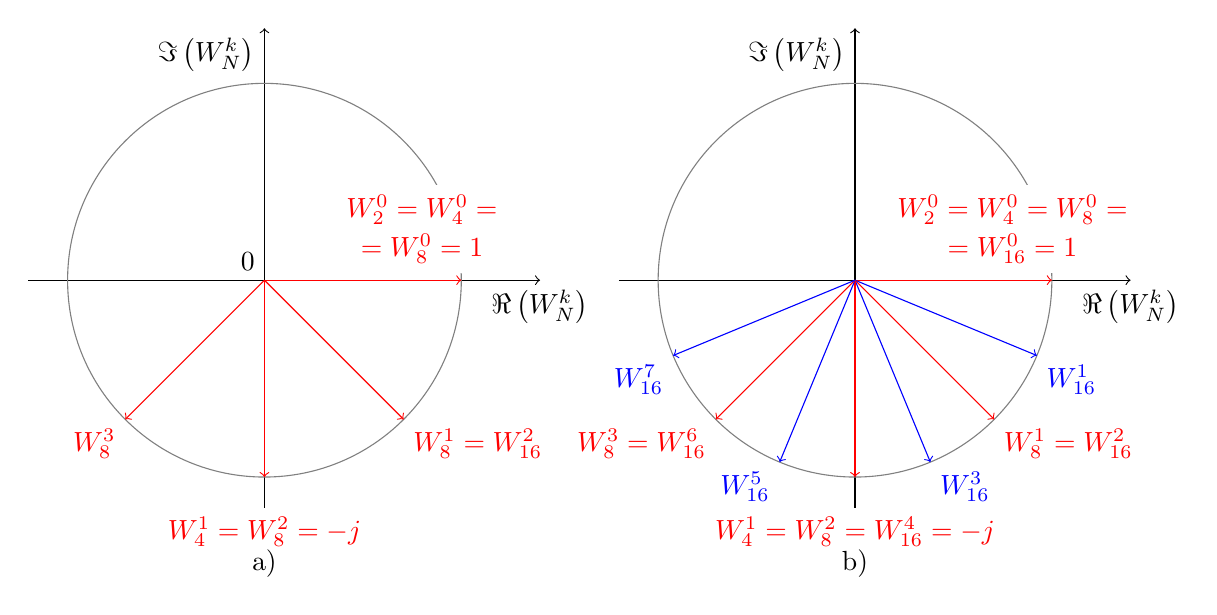
\begin{tikzpicture}

\draw[->] (-3, 0) -- (3.5,0) node[below]{$\Re\left(W_N^k\right)$};
\draw[->] (0, -3) -- (0,3.2) node[below left]{$\Im\left(W_N^k\right)$};


\draw[->] (4.5, 0) -- (11,0) node[below]{$\Re\left(W_N^k\right)$};
\draw[->] (7.5, -3) -- (7.5,3.2) node[below left]{$\Im\left(W_N^k\right)$};

\draw[gray, thin] (0,0) circle (2.5);
\draw[gray, thin] (7.5,0) circle (2.5);


\draw[->, red] (0:0) -- (0:2.5);	
\draw[red] (2, 0.9) node[fill=white] {$W_2^0 =W_4^0 = $} ;
\draw[red] (2, 0.4) node[fill=white] {$ = W_8^0 = 1$} ;


\draw[->, red] (7.5,0) -- (10,0);	
\draw[red] (9.5, 0.9) node[fill=white] {$W_2^0 =W_4^0=W_8^0 = $} ;
\draw[red] (9.5, 0.4) node[fill=white] {$ = W_{16}^0 = 1$} ;

\draw[->, blue, rotate around={-22.5:(7.5,0)}] (7.5,0) -- (10, 0) node[below right] {$W_{16}^1$};
\draw[->, red, rotate around={-45:(7.5,0)}] (7.5,0) -- (10, 0) node[below right] {$W_8^1 = W_{16}^2$};

\draw[->, blue, rotate around={-67.5:(7.5,0)}] (7.5,0) -- (10, 0) node[below right] {$W_{16}^3$};

\draw[->, red, rotate around={-90:(7.5,0)}] (7.5,0) -- (10, 0); 

\draw[red] (7.5, -3.2) node[fill = white] {$W_4^1 = W_{8}^2 = W_{16}^4 = -j$};

\draw[->, blue, rotate around={-112.5:(7.5,0)}] (7.5,0) -- (10, 0) node[below left] {$W_{16}^5$};

\draw[->, red, rotate around={-135:(7.5,0)}] (7.5,0) -- (10, 0) node[below left] {$W_8^3 = W_{16}^6$};

\draw[->, blue, rotate around={-157.5:(7.5,0)}] (7.5,0) -- (10, 0) node[below left] {$W_{16}^7$};



\draw[->, red] (0:0) -- (-45:2.5) node[below right] {$W_8^1 = W_{16}^2$};
\draw[->, red] (0:0) -- (-90:2.5) ;
\draw[red] (0, -3.2) node[fill=white] {$W_4^1 = W_8^2 = -j$};
\draw[->, red] (0:0) -- (-135:2.5) node[below left] {$W_8^3$};
\draw (0,0) node[above left] {$0$};


\draw(0, -3.6) node {a)};
\draw(7.5, -3.6) node {b)};

\end{tikzpicture}

\end {document}




